\section{Metodología y resultados}
Las secciones anteriores han servido para motivar y explicar este trabajo y para tener una base teórica sólida que nos proporcionará las herramientas necesarias para hacer los cálculos. Ahora, introduciremos la metodología utilizada y los resultados de las simulaciones. En primer lugar, determinaremos la distancia entre átomos de carbono de la red de grafeno que utilizará el código FIREBALL para comprobar que es compatible con el valor experimental de 1.42 \AA. Posteriormente, procederemos a simular una celda de tamaño 18x8 de 288 átomos de carbono y estiraremos en pasos sucesivos (desplazamientos de $0.1$ \AA\ de los átomos en cada paso), siempre en la dirección \emph{armchair}, de diferentes maneras (4 casos):
\begin{enumerate}
    \item Estirando en direcciones opuestas de forma rígida por los extremos y permitiendo la relajación (reestructuración de átomos para minimización de la energía) de la red en la región central.
    \item Estirando en direcciones opuestas por la mitad de la red, permitiendo la relajación de la estructura en la región central de la red. 
    \item Estirando de forma rígida los extremos de la red (como en el caso 1) y de forma proporcional a la distancia del centro de la red en la región central.
    \item Estirando de forma idéntica al caso 1 y, al quedar pocos pasos para una ruptura, intercalamos pasos de dinámica molecular (movimiento libre de átomos por acción de la temperatura) y de relajación de la estructura con el estiramiento.
\end{enumerate}
Además de diferentes estiramientos, se introducirán impurezas, como boro o nitrógeno, o defectos, como una vacante y una divacante, en la posición central de la red mientras se estira como en el caso 1. 
\begin{figure}[htbp]
    \centering
    \def\svgwidth{.65\textwidth}
    \input{regiones_graf.pdf_tex}
    \caption{Red de grafeno 18x8 y regiones central y de extremos. La región central tiene un tamaño de 10x8 ($16a$ en la dirección \arm) y los extremos de 4x8 cada uno ($10a$). La celda entera contiene 288 átomos de carbono.}
    \label{fig:enter-label}
\end{figure}

\subsection{Grafeno 1x1 y distancia carbono-carbono}

\begin{figure}[htbp]
    \centering
    \begin{subfigure}{0.41\textwidth}
        \centering
        \def\svgwidth{.8\textwidth}
        \input{base_vdirecta.pdf_tex}
        \caption{Base de grafeno (red directa).}
    \end{subfigure}
    \begin{subfigure}{0.41\textwidth}
        \centering
        \def\svgwidth{.8\textwidth}
        \input{vreciproca.pdf_tex}
        \caption{Primera zona de Brillouin del grafeno.}
    \end{subfigure}
    \caption{Vectores de la red directa $\{ \B{a}_i \}$ y de la red recíproca $\{ \B{b}_i \}$.}
    \label{fig:4.2}
\end{figure}

El objetivo principal, como hemos venido diciendo, es estudiar los efectos del estiramiento en la red de grafeno para determinar sus propiedades mecánicas y elásticas. Antes de ponernos a simular una red de grafeno de gran tamaño, lo ideal es asegurarnos de que nuestro programa toma valores razonables para la distancia de carbono-carbono. La base de grafeno es, como ya hemos visto, hexagonal, con vectores de red $\B{a}_1$ y $\B{a}_2$ que son
\begin{equation}
    \B{a}_1 = a/2 (\sqrt{3}, 1) \quad , \quad \B{a}_2 = a/2 (-\sqrt{3},1) \ .
\end{equation}
La red recíproca tiene como vectores de red a $\B{b}_1$ y $\B{b}_2$, 
\begin{equation}
    \B{b}_1 = \frac{2\pi }{3a} (\sqrt{3}, 1) \quad , \quad \B{b}_2 = \frac{2\pi }{3a} (-\sqrt{3},1) \ .
\end{equation}
En el caso del grafeno, sabemos que $d = 1.42$ \AA; pero FIREBALL, debido a las aproximaciones realizadas, utilizará un valor ligeramente distinto, como veremos a continuación. Comenzaremos realizando unas simulaciones de la base de grafeno de dos átomos de carbono fijos, y variaremos su distancia interatómica en cada simulación para determinar qué parámetro de red minimiza la energía. El resultado es el siguiente.

\begin{figure}[!h]
    \centering
    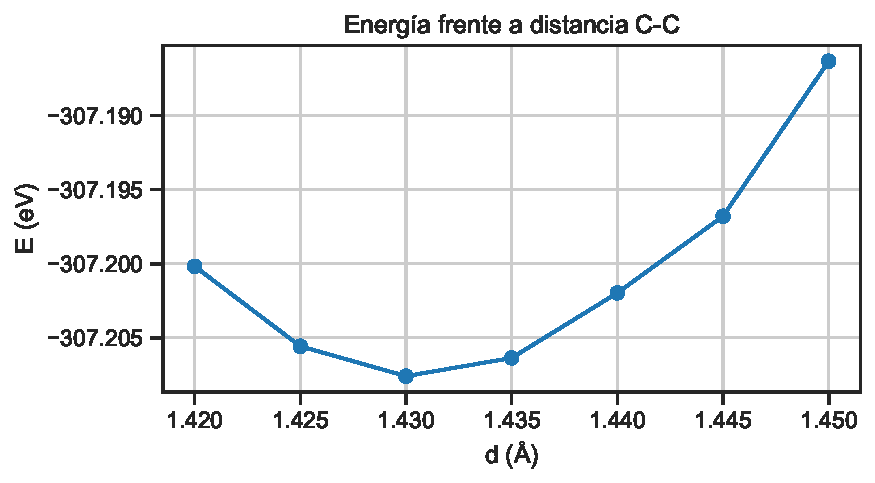
\includegraphics[width = .7\linewidth]{ADJUNTOS/En_param_graf1x1.pdf}
    \caption{Curva de energía de la base de grafeno (1x1) frente a la distancia carbono-carbono. La energía se minimiza para el valor $d = 1.43$ \AA.}
    \label{fig:4.3}
\end{figure}

El valor de la distancia entre carbonos que minimiza la energía -- y que definirá, por lo tanto, a nuestra base de grafeno -- es de $1.43$ \AA\  (error del $0.7\%$). Podemos terminar de verificar que este es el valor apropiado si calculamos la densidad de estados en cualquiera de los átomos de la base. Como puede verse en la Figura \ref{fig:4.4}, distinguimos el ya mencionado cono de Dirac en el nivel de Fermi de la celda 1x1, lo cual confirma que el parámetro tomado por FIREBALL reproduce de forma fiable los resultados teóricos.

\begin{figure}[!h]
    \centering
    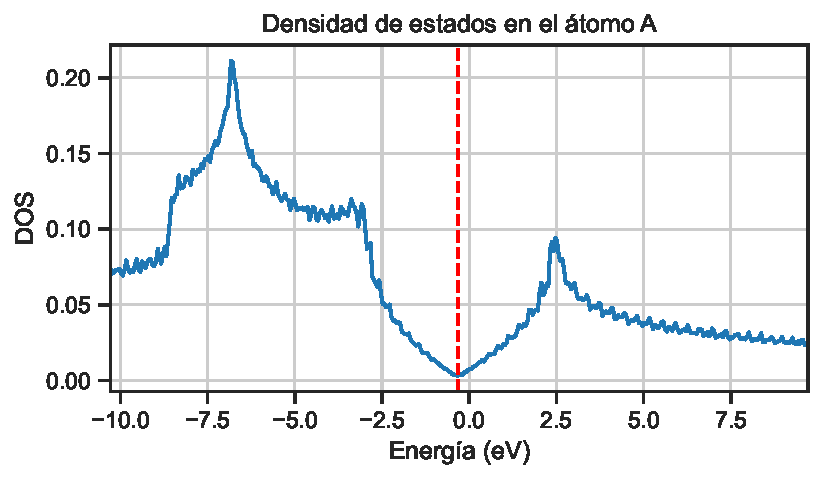
\includegraphics[width = .6\linewidth]{DOS_1x1.pdf}
    \caption{Densidad de estados calculada en el átomo A (ver Figura \ref{fig:4.2}). La línea discontinua representa el nivel de Fermi, $E_F = -0.279$ eV.}
    \label{fig:4.4}
\end{figure}


\subsection{Grafeno 18x8}

Una vez comprobado que la distancia entre carbonos es apropiada para realizar cálculos, podemos comenzar a simular una red de grafeno de mayor tamaño. La red 18x8 tiene como vectores de red:

\begin{equation}
    \B{u}_1 = a (27,0)\quad , \quad \B{u}_2 = a (0,8\sqrt{3}) \quad {\text{\small (dirección \arm orientada en $x$)}}
\end{equation}

En primer lugar, estudiaremos la energía del estado fundamental del grafeno conforme realizamos estiramientos, siguiendo la metodología mencionada anteriormente. 

\subsubsection{Estiramiento rígido} \label{er}
Comenzaremos simulando el estiramiento desplazando de forma rígida los extremos en direcciones opuestas. Cada estiramiento supondrá un desplazamiento en la dirección \arm de $0.1$ \AA \ con respecto a su posición original. De este modo, para cada simulación tomaremos una red desplazada $0.2$ \AA \ con respecto al paso anterior, lo que nos permitirá observar una evolución suave de la energía de la red. Para alcanzar la ruptura, realizamos 26 estiramientos de la red. Dado el gran número de átomos, un número apropiado de puntos $k$ especiales para la relajación (y que no prolongue de forma innecesaria el tiempo de simulación) es de 4 puntos. La energía frente al desplazamiento de la red se puede observar en la Figura \ref{fig:4.5} (a). 
\captionsetup[subfigure]{font={small}, skip=1pt, margin=1cm, singlelinecheck=false}
\begin{figure}[!h]
    \centering
    \begin{subfigure}{0.5\textwidth}
        \caption{}
        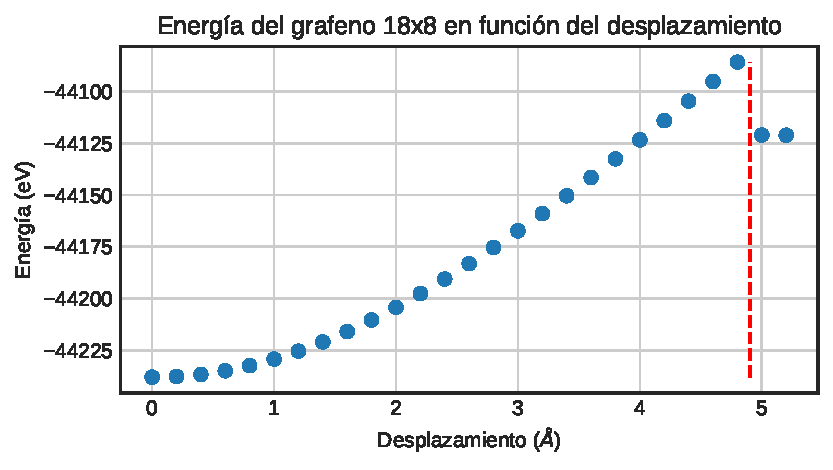
\includegraphics[width = \linewidth]{ADJUNTOS/graf_18x8_en.pdf}
    \end{subfigure}
    \begin{subfigure}{0.487\textwidth}
        \caption{}
        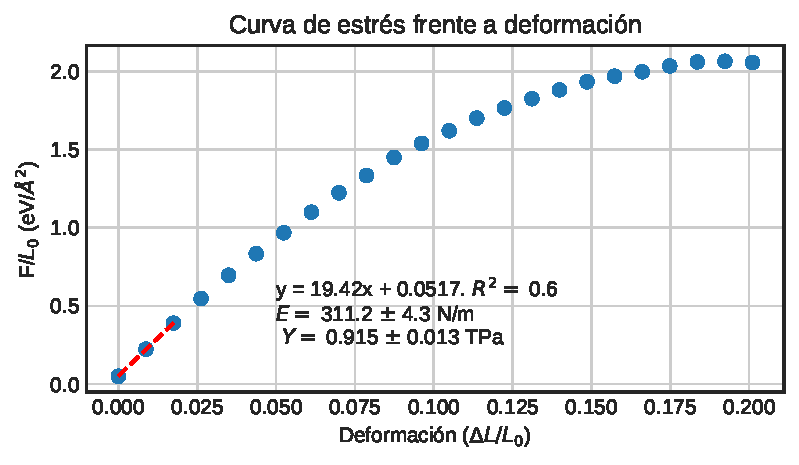
\includegraphics[width = \linewidth]{ADJUNTOS/graf_18x8_young.pdf}
    \end{subfigure}
    \caption{Comportamiento mecánico de la red de grafeno 18x8. a) Energía frente al desplazamiento de la red, b) Estrés frente a deformación de la red. }
    \label{fig:4.5}
\end{figure}

Observamos que, conforme progresan los estiramientos, la energía aumenta hasta un valor máximo, a partir del cual la energía disminuye repentinamente, que coincide con el punto en el cual se alcanza la ruptura de la red. El comportamiento de la energía al estirar el grafeno puede interpretarse dentro de la teoría de elasticidad lineal. Podemos distinguir dos regímenes para la energía: régimen de deformación lineal o simplemente régimen elástico, en el cual las deformaciones aplicadas sobre el grafeno son reversibles y la red retorna a su longitud inicial; y de ruptura, donde se pierde esta reversibilidad y los cambios en la red son permanentes. La fuerza efectiva aplicada sobre la red al modificar las posiciones de los átomos puede tomarse como conservativa y calcularse diferenciando la energía con respecto al desplazamiento. Esta fuerza o estrés ($\sigma$, fuerza partida por la longitud original $L_0$ de la región central\footnote{En materiales 3D, el estrés viene definido como la fuerza por unidad de área transversal a la deformación.}) frente a la deformación $\varepsilon = \Delta L/L_0$ se representa en la Figura \ref{fig:4.5} (b). En la gráfica, observamos que la ruptura se produce para una deformación del 20$\%$ y para un estrés máximo de $32.94$ N/m, que está en acuerdo con resultados previos realizados en DFT\footnote{Cálculos realizados con Quantum Espresso (QE), un código de simulación más preciso pero más lento.} tanto para deformaciones en la dirección \arm como en la \zig \cite{elastic}. El estrés aplicado sobre el material se relaciona con la deformación, en régimen lineal (estrés y deformaciones pequeñas), con el módulo de Young como $\sigma = E \varepsilon$. Por tanto, podemos obtener el módulo de Young (en dos dimensiones) del grafeno como la pendiente de la curva para deformaciones pequeñas, que toma un valor $E = 311$ N/m para nuestras simulaciones. El módulo de Young efectivo puede calcularse finalmente como $Y = E/t$, donde $t$ es el grosor de la red de grafeno\footnote{Tomado como la distancia entre dos láminas de grafito.}. Tomando $t = 3.4$ \AA \ , $Y = 0.915$ TPa. Existen muchos estudios computacionales de las propiedades mecánicas del grafeno que, en función del código de simulación o el modelo físico utilizado para realizar los cálculos (dinámica molecular, modelos continuos, etc.), brindan valores para el módulo de Young distintos. El valor experimental calculado en 2008 \cite{science} se encuentra en $1.0 \pm 0.1 $ TPa, mientras que los métodos computacionales proporcionan valores que se encuentran entre los 0.6 y 1.4 TPa \cite{MEMARIAN2015348}. A pesar de que los ajustes realizados brindan valores del módulo de Young coherentes con los experimentales y son compatibles con los obtenidos mediante otros modelos de simulación, la poca cantidad de datos utilizados no nos permite afirmar con confianza que sean resultados fiables, por lo que un número mayor de puntos (tomando, por ejemplo, más estiramientos con menor desplazamiento) sería más apropiado.\\

Si bien es cierto que, para pequeñas fuerzas aplicadas y pequeñas deformaciones, los materiales presentan un régimen lineal, un análisis más exhaustivo debería tener en cuenta la respuesta mecánica no lineal del grafeno. Este modelo, adoptado por ejemplo en el resultado de Lee \cite{science}, tiene en cuenta órdenes superiores de deformación, teniendo que la tensión mecánica en la dirección \arm es
\begin{equation}
    \sigma = Y \varepsilon + D \varepsilon^2
\end{equation}
donde $Y$ es el módulo de Young y $D$ el módulo elástico de tercer orden. Realizando este ajuste polinómico a todos los datos, obtenemos un valor de $325.9 \pm 1.4$ N/m para el módulo de Young en dos dimensiones y $D = -824.7 \pm 6.5$ N/m (en dos dimensiones), por lo que el módulo efectivo $Y = 0.9584 \pm 0.0040$ TPa, que es una mejoría con respecto a los resultados anteriores, si bien el valor para la constante elástica de tercer orden en dos dimensiones es más pequeña que el valor experimental ($-690 $ N/m), lo cual no es fuera de lo común ya que FIREBALL sobre-estima las interacciones. 

Centrándonos en la estructura resultante después de los estiramientos, en las Figuras \ref{fig:4.19} y \ref{fig:4.6} se puede observar la estructura de grafeno en un paso intermedio de estiramiento y tras la ruptura de la red. 

\begin{figure}[!h]
    \centering
    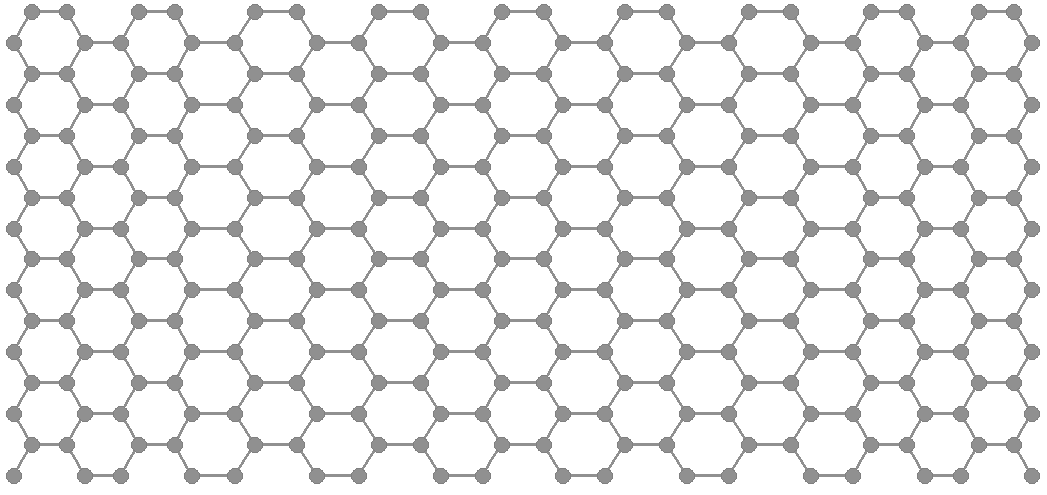
\includegraphics[width = .6\linewidth]{ADJUNTOS/grafeno_a_punto.png}  
    \caption{Estiramiento intermedio. Deformación de la red en la región central.}
    \label{fig:4.19}
\end{figure}
\begin{figure}[!h]
    \centering
    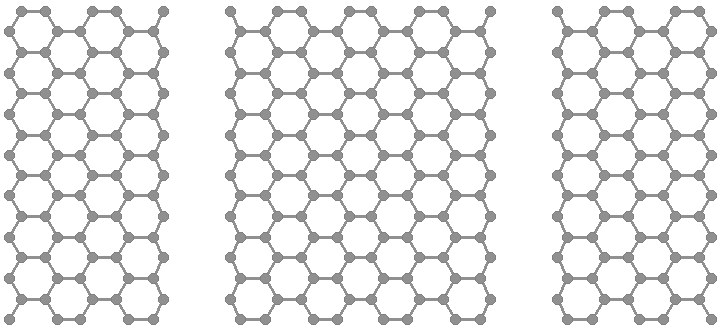
\includegraphics[width = .6\linewidth]{ADJUNTOS/grafeno_roto.png}
    \caption{Red después de la ruptura. Se produce de forma simétrica en ambos extremos.}
    \label{fig:4.6}
\end{figure}

Como era de esperar, la ruptura de la red se produce cerca de la frontera entre el extremo y la región central, que es donde hay una ruptura de la simetría de la red hexagonal. Se produce además de forma simultánea en ambos extremos al producirse el estiramiento de forma simétrica.\\


Por último, podemos comparar la densidad de estados de los átomos de la región central para observar un cambio en las propiedades electrónicas del grafeno (calculando con 64 puntos $k$ especiales). En concreto, consideramos dos estiramientos, uno intermedio (con distancia entre átomos de carbono del centro de la red $d = 1.65$ \AA) y otro pocos pasos antes de la ruptura ($d = 1.75$ \AA), y comparamos con la densidad de estados teórica del grafeno sin estirar . Como puede comprobarse en la Figura \ref{fig:4.16}, el estiramiento tiene el efecto de modificar la densidad de estados, teniendo un valor no nulo en el nivel de Fermi y formándose un gap, si bien las curvas de densidad de estados tienen bastante distorsión. Esto es debido a que se ha utilizado un número de puntos $\B{k}$ de la primera zona de Brillouin insuficientes, lo cual genera ondulaciones en las curvas de DOS. Para poder determinar con precisión esta apertura de gap, sería necesario recalcular las densidades de estados con mayor número de puntos (esto es, dedicando un mayor tiempo de cómputo).  


\begin{figure}[!h]
    \centering
    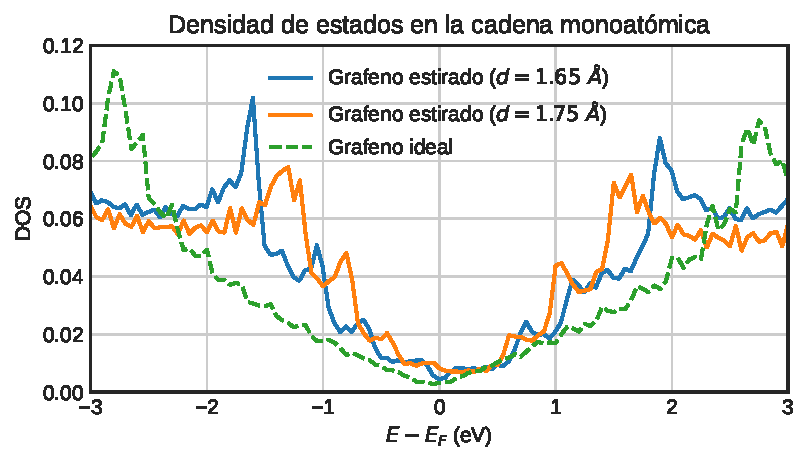
\includegraphics[width = .7\linewidth]{ADJUNTOS/DOS_graf18x8_int_av_141.pdf}
    \caption{Efecto del estiramiento en la densidad de estados del grafeno. }
    \label{fig:4.16}
\end{figure}

\subsubsection{Comparación de métodos de estiramiento}
En la siguiente sección comentamos la estabilidad que tienen diferentes métodos de estiramiento en comparación con el estiramiento por los extremos de forma rígida. En concreto, analizamos dos formas de estirar alternativas: desplazando la red por mitades en direcciones opuestas y relajando la red, manteniendo fijos los átomos de los extremos; y estirando por los extremos de forma rígida además de desplazar los átomos de la región central en direcciones contrarias un pequeño porcentaje (que es proporcional a la distancia a los extremos), dejando que la estructura relaje fijando los extremos como anteriormente. El primer método (estiramiento por el centro) nos permite distinguir si resulta más viable energéticamente romper la simetría en otra parte de la red que en los extremos; y el segundo nos permite simular un caso de estiramiento progresivo ligeramente más realista que el caso de un desplazamiento repentino únicamente de los extremos. Para este último, los átomos del centro de la red permanecerán inmóviles mientras que el resto se desplazarán en incrementos del $10\%$ del desplazamiento original (que es $0.1$ \AA. Es decir, $0.01$ \AA \ para la primera columna de átomos, $0.02$ \AA \ la segunda, etc.). En la Figura \ref{fig:4.7} se ven representadas las energías (respecto a su energía inicial) para los tres métodos mencionados para 20 estiramientos (desplazamiento total de $4$ \AA).  \\

\begin{figure}[!h]
    \centering
    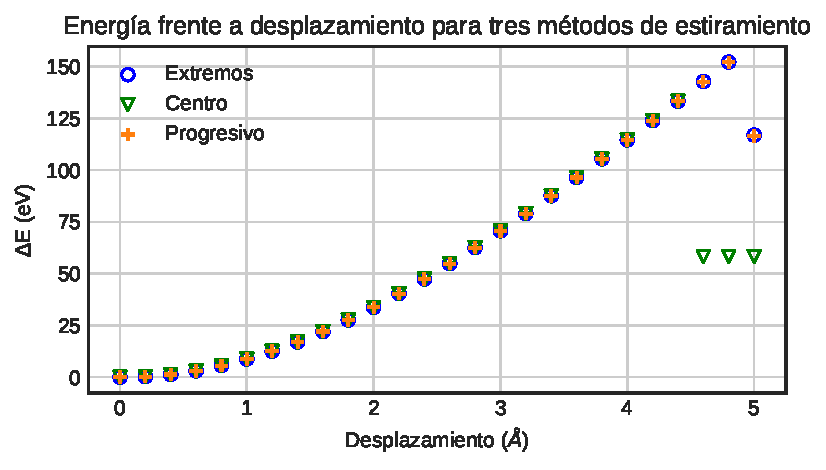
\includegraphics[width = .7\linewidth]{ADJUNTOS/graf_18x8_comp_en.pdf}
    \caption{Comparación de métodos de estiramiento de la red de grafeno 18x8.}
    \label{fig:4.7}
\end{figure}

\begin{figure}[!h]
    \centering
    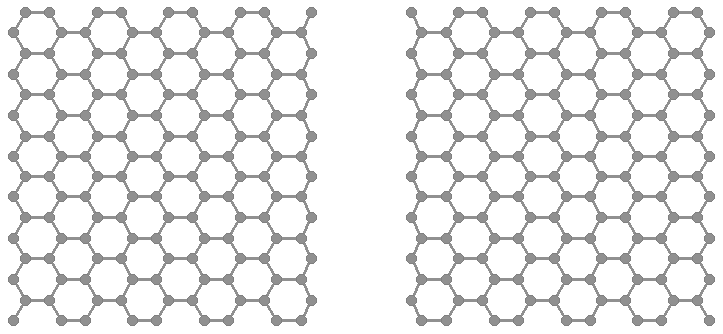
\includegraphics[width = .6\linewidth]{ADJUNTOS/roto_centro.png}
    \caption{Estructura final tras estirar por el centro de la red.}
    \label{fig:4.8}
\end{figure}

Como se puede comprobar, la energía en las primeras etapas del estiramiento es la misma independientemente de qué método de estiramiento escojamos. Este resultado es lo esperable ya que, al no modificarse en gran medida la forma de la estructura, la relajación de la red después de estirar acaba por retornar el mismo estado fundamental en los tres casos, distribuyendo la deformación entre todos los enlaces. No obstante, al estirar por el centro la red acaba por romperse antes, acabando en un estado de mucha menor energía que en los dos casos anteriores. Si observamos la estructura final (Figura \ref{fig:4.8}) estirando por el centro, vemos que la ruptura se produce en el centro de la red. En el caso del estiramiento por los extremos, acabamos rompiendo dos cadenas de enlaces, dando lugar a tres subsistemas; mientras que en este estiramiento solo rompemos una cadena de enlaces. Es lógico por tanto concluir que el método de estiramiento de la red más estable es por el centro.

\subsubsection{Estiramiento con dinámica molecular}

El último método de estiramiento que consideramos en este trabajo combina el estiramiento de la red por los extremos con pasos de dinámica molecular para desorganizar la red antes de cada estiramiento. Las simulaciones realizadas anteriormente, si bien son coherentes con lo esperado a temperatura nula, no reflejan de forma adecuada la situación real de deformación de una lámina de grafeno, en la cual la temperatura, ya no nula, juega un papel central en la reorganización de la red para la minimización de la energía al introducir asimetrías puntuales, que pueden llevarnos a situaciones de ruptura distintas. Para simular este estiramiento realista, realizamos estiramientos centrales vistos anteriormente hasta que la red se encuentre cerca de la ruptura. A partir de este punto, introducimos una temperatura (600 K) y dejamos evolucionar el sistema de forma libre durante una serie de pasos (500). Posteriormente, relajamos la estructura y continuamos estirando y relajando. Repetimos este proceso de dinámica molecular-relajación-estiramiento-relajación hasta alcanzar la ruptura de la red. Los resultados de este procedimiento se ven en las Figuras \ref{fig:4.9} y \ref{fig:4.10}. \\

Lo primero que observamos al analizar las energías es que la ``ruptura'' se produce antes estirando y desorganizando la red por dinámica molecular que si solamente estiramos por los extremos. La energía durante los últimos pasos son iguales en ambos casos, pero las energías después de la ruptura en ambos casos indican que el estiramiento con pasos de dinámica nos lleva a estructuras más estables que en caso contrario. \\

\begin{figure}[!h]
    \centering
    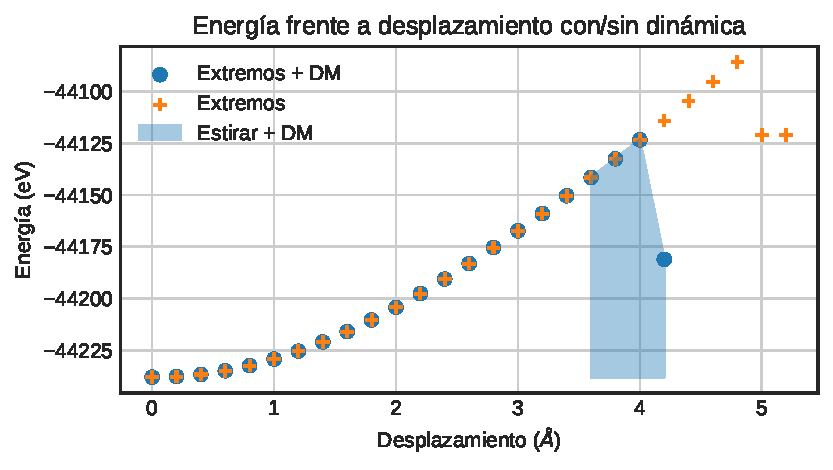
\includegraphics[width = .7\linewidth]{ADJUNTOS/graf_18x8_v5_en.pdf}
    \caption{Comparación de energía estirando con y sin dinámica molecular (MD).}
    \label{fig:4.9}
\end{figure}

\begin{figure}[!h]
    \centering
    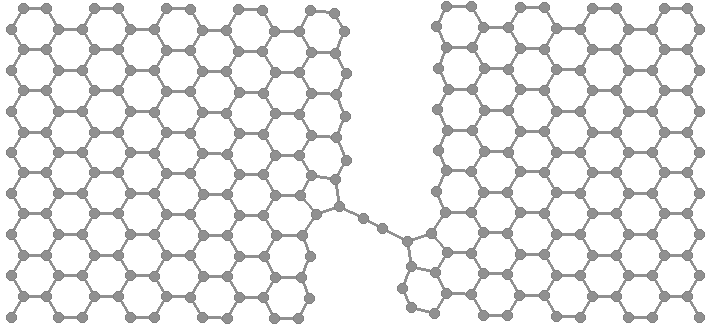
\includegraphics[width = .6\linewidth]{ADJUNTOS/cadena-mono.png}
    \caption{Red de grafeno tras estirar con dinámica molecular y formación de una cadena monoatómica.}
    \label{fig:4.10}
\end{figure}

Lo más interesante de este método de estiramiento es la estructura final resultante. En este caso, podemos ver que la ruptura de la red está incompleta y que se ha formado una cadena monoatómica entre ambas secciones. Es un resultado completamente distinto al de los otros tres métodos de estiramiento pero que es más coherente con una situación realista de estiramiento de grafeno, en la que el efecto de la temperatura reordena los átomos permitiendo que alcancen nuevas configuraciones de mínima energía, en este caso una cadena de átomos. Dado que la dinámica molecular es un proceso inherentemente aleatorio, al volver a simular este procedimiento es posible que obtengamos una estructura distinta de la observada. Esto puede dar paso a seguir estudiando la formación de estas estructuras, repitiendo las simulaciones para mismas condiciones y poder así hacer estadística o en diferentes condiciones de estiramiento y de temperatura para explorar nuevas posibles estructuras. \\

Podemos fijarnos en la densidad de estados en los átomos de la cadena monoatómica, como se ve en la Figura \ref{fig:4.17}. Nos encontramos con un gran pico de densidad en la región cercana al nivel de Fermi. La presencia de este pico tiene consecuencias en las propiedades electrónicas de la cadena de átomos, ya que, al haber electrones ocupando estados cercanos al nivel de Fermi, se puede dar la posibilidad de conducción entre ambas regiones conectadas por la cadena monoatómica; además de hacer la cadena reactiva, por lo que otra futura línea de trabajo puede ser estudiar la interacción de esta estructura con otros átomos o moléculas. \\

\begin{figure}[!h]
    \centering
    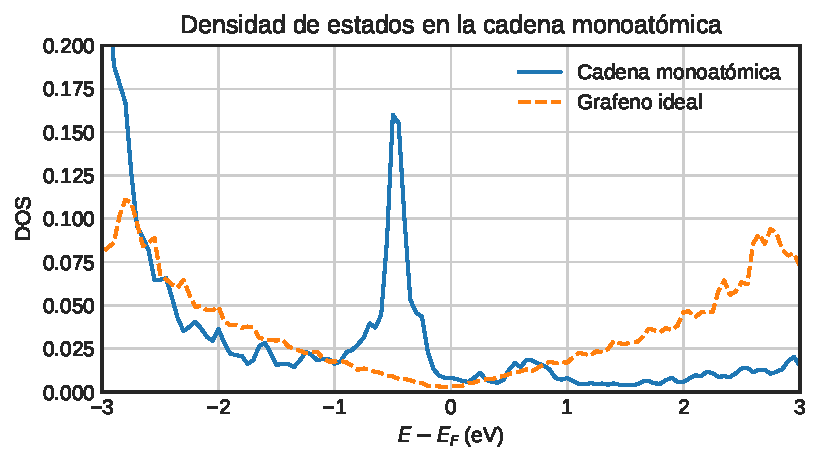
\includegraphics[width = .7\linewidth]{ADJUNTOS/DOS_graf18x8_cadena.pdf}
    \caption{Densidad de estados en la cadena monoatómica.}
    \label{fig:4.17}
\end{figure}

\subsection{Grafeno 18x8 con defectos}
En esta sección, analizaremos el efecto de introducir dos defectos en la red en sus propiedades mecánicas. En este caso, introducimos una vacante y divacante (uno y dos huecos) en la red y estiramos por los extremos hasta alcanzar la ruptura. Los resultados se ilustran en las Figuras \ref{fig:4.11}, \ref{fig:4.14} y \ref{fig:4.15}. \\

\begin{figure}[!h]
     \centering
     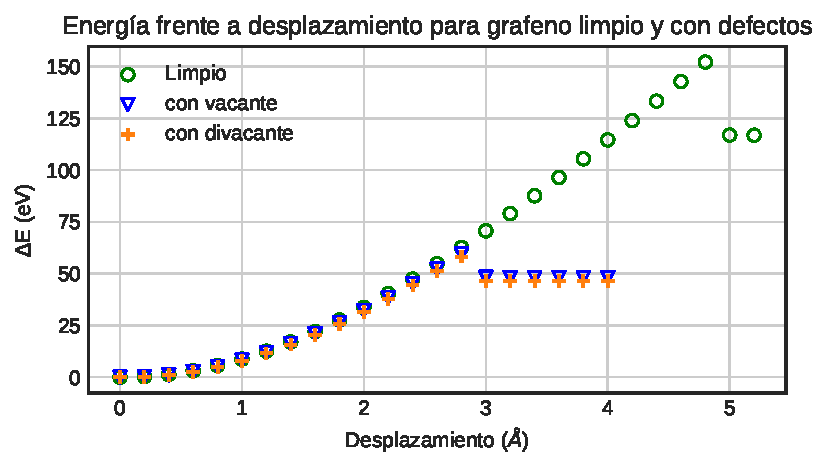
\includegraphics[width = 0.7\linewidth]{ADJUNTOS/graf_18x8_v1-vac-divac_en.pdf}
     \caption{Comparación de energías del grafeno ``limpio'' y con vacante y divacante.}
     \label{fig:4.11}
 \end{figure}

\begin{figure}[!h]
    \centering
    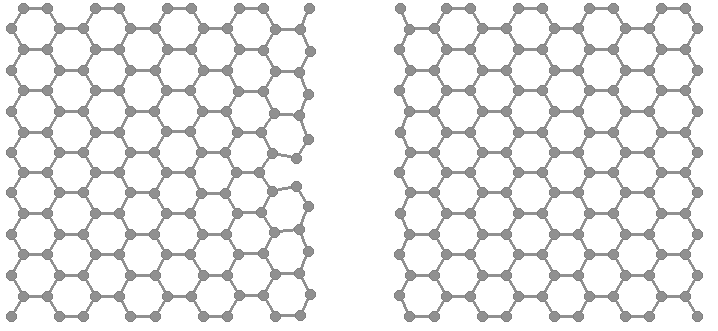
\includegraphics[width = .6\linewidth]{ADJUNTOS/roto_vacante.png}
    \caption{Estructura final de la red de grafeno con una vacante}
    \label{fig:4.14}
\end{figure}

\begin{figure}[!h]
    \centering
    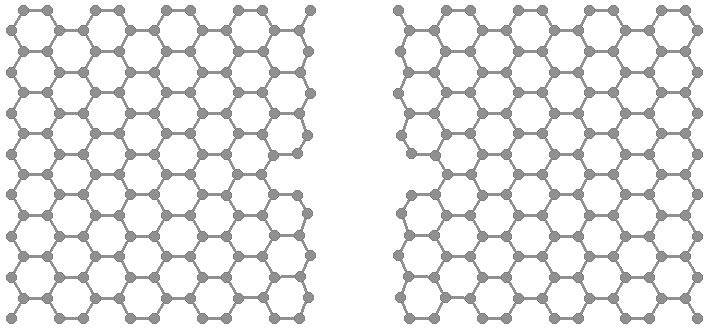
\includegraphics[width = .6\linewidth]{ADJUNTOS/roto_divacante.png}
    \caption{Estructura final de la red de grafeno con dos vacantes. }
    \label{fig:4.15}
\end{figure}

La progresión de la energía es muy similar para la red de grafeno limpia como para las redes con defectos. La ruptura, sin embargo, se produce mucho antes en el caso de la red con defectos que en la red normal, alcanzándose en ambos casos a $3.0$ \AA \ de elongación con respecto a la longitud inicial. De hecho, esta ruptura se produce incluso antes que en el caso del boro ($4.2$ \AA) y del nitrógeno ($3.8$ \AA), como veremos más adelante. Esto es debido a que, con dopantes, existen enlaces -- si bien son débiles -- con el carbono que desaparecen al introducir una vacante (3 en el caso de la vacante, 6 con la divacante). Esto genera una cierta inestabilidad estructural que favorece la ruptura de la red. Calculando el módulo de Young efectivo (en el caso de la divacante), obtenemos un valor de $Y = 0.892 \pm 0.016 $ TPa, ligeramente inferior al de la red ideal, mientras que con el ajuste cuadrático obtenemos un módulo efectivo de $0.974 \pm 0.020$ TPa. La disparidad entre ambos valores para la divacante puede deberse a la falta de puntos a mayores deformaciones debido a la temprana ruptura de la red, por lo que sería necesario un cálculo con menor desplazamiento en cada estiramiento.


\subsection{Grafeno 18x8 dopado}

Finalmente, estudiaremos el efecto de dopar la red de grafeno con un átomo de boro o de nitrógeno mientras estiramos por los extremos. Tanto el boro, con tres electrones en su capa de valencia, como el nitrógeno, con cinco electrones, cambiarán la distribución de las cargas de la región próxima al dopante, de manera que la simetría entre los enlaces con los carbonos se romperá y generarán una inestabilidad que tendrá consecuencias en el estiramiento de la red. En ambos casos, el dopante sustituirá al átomo de la posición central de la red, y se procederá a estirar el retículo de la misma forma que se planteó en la sección \ref{er}. Los resultados tanto para el boro como para el nitrógeno se representan en la Figura \ref{fig:4.11}.
 \begin{figure}[!h]
     \centering
     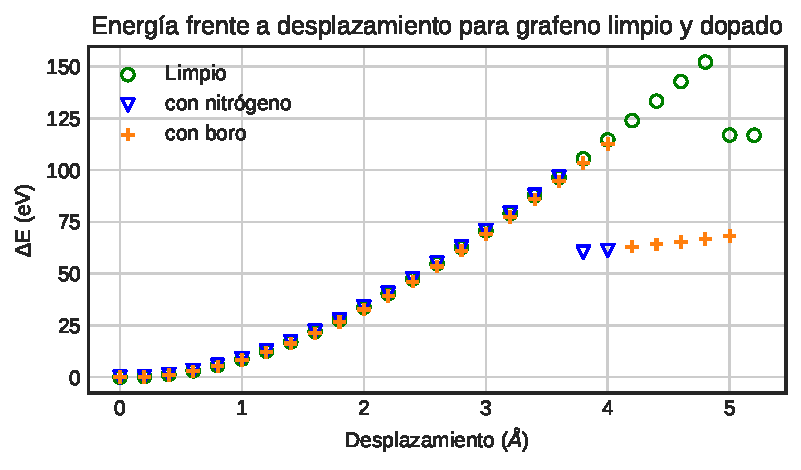
\includegraphics[width = 0.7\linewidth]{ADJUNTOS/graf_18x8_v1-nit-bor_en.pdf}
     \caption{Comparación de energías del grafeno ``limpio'' y dopado con boro y nitrógeno.}
     \label{fig:4.11}
 \end{figure}
En la gráfica vemos que la progresión de la energía para las tres redes de grafeno son muy parecidas hasta el estiramiento $\#$18, a partir del cual el grafeno con nitrógeno se rompe; seguido del boro dos pasos después. Vemos entonces que dopar la red de grafeno, si bien es estable, acaba rompiéndose antes debido a esta ruptura de simetría. Un cálculo de estrés en la red por deformación como en la sección \ref{er} nos permite calcular el módulo de Young efectivo de la red con boro y con nitrógeno, dando como resultado $0.921 \pm 0.019$ TPa para el caso del boro y de $0.917 \pm 0.015$ TPa. Un ajuste cuadrático a la curva entera nos proporciona los siguientes valores: para el nitrógeno, $0.9623 \pm 0.0076$ TPa y para el boro, $0.9505 \pm 0.0094$ TPa, que son ambos muy cercanos al valor de la red de grafeno limpio.\\

Fijándonos en las estructuras resultantes (Figuras \ref{fig:4.12} y \ref{fig:4.13}), vemos que en ambos casos la estructura se rompe por el centro de la red, en la región del dopante. Este resultado, como hemos comentado antes, se debe a la ruptura de la simetría de la red en el enlace boro-carbono o nitrógeno-carbono, haciendo que sea más beneficioso energéticamente romper la red por el centro en vez de los extremos, como en el caso del grafeno limpio. Por último, vemos también que, en ambos casos, se forman cadenas de átomos de carbono en las partes más alejadas del dopante en la zona de la ruptura. Como en el caso de dinámica molecular con el grafeno limpio, puede ser interesante seguir estudiando la formación de estas cadenas en diferentes condiciones de estiramiento e introduciendo temperatura, además de sus propiedades electrónicas. 

\begin{figure}[!h]
    \centering
    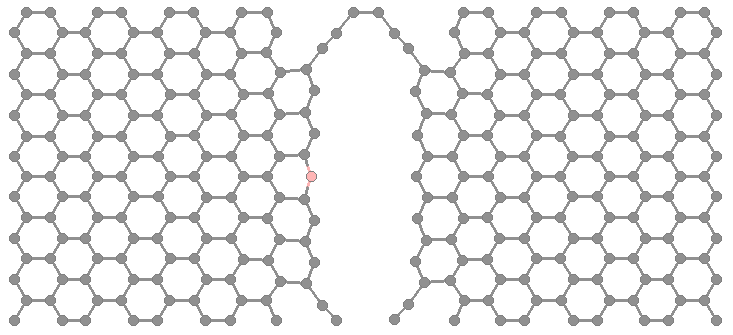
\includegraphics[width = .6\linewidth]{ADJUNTOS/roto_boro.png}
    \caption{Estructura final de grafeno con boro.}
    \label{fig:4.12}
\end{figure}

\begin{figure}[!h]
    \centering
    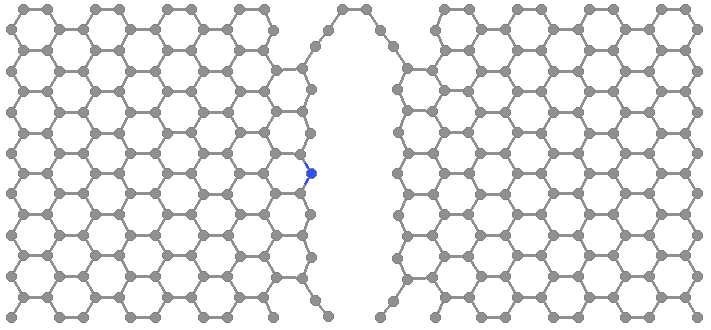
\includegraphics[width = .6\linewidth]{ADJUNTOS/roto_nitro.png}
    \caption{Estructura final de grafeno con nitrógeno.}
    \label{fig:4.13}
\end{figure}



% \subsection{Grafeno 18x8 con defectos}
% De la misma manera que con los dopantes, introduciremos dos defectos en la red para estudiar sus propiedades mecánicas. En este caso, introducimos una vacante y divacante (uno y dos huecos) en la red y estiramos por los extremos hasta alcanzar la ruptura. Los resultados se ilustran en las Figuras \ref{fig:4.11}, \ref{fig:4.14} y \ref{fig:4.15}. \\

% \begin{figure}[!h]
%      \centering
%      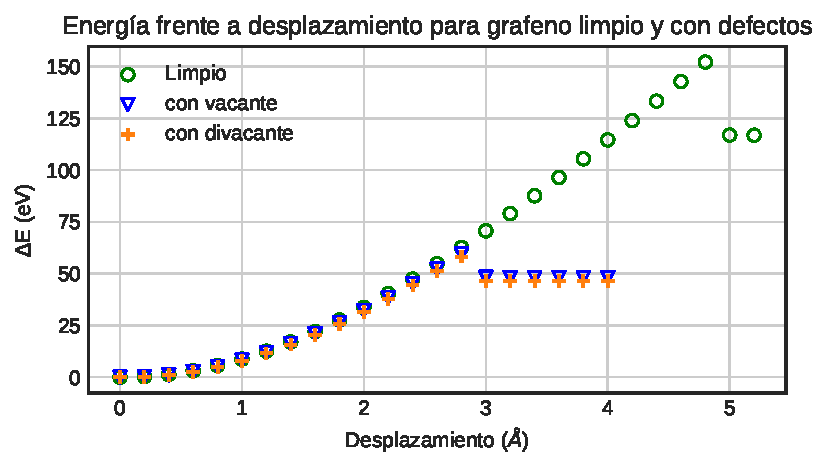
\includegraphics[width = 0.7\linewidth]{ADJUNTOS/graf_18x8_v1-vac-divac_en.pdf}
%      \caption{Comparación de energías del grafeno ``limpio'' y con vacante y divacante.}
%      \label{fig:4.11}
%  \end{figure}

% \begin{figure}[!h]
%     \centering
%     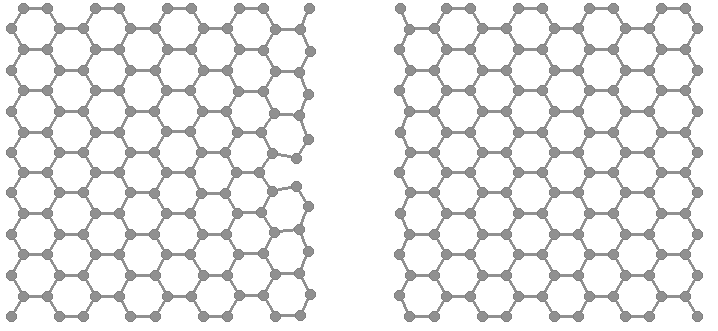
\includegraphics[width = .6\linewidth]{ADJUNTOS/roto_vacante.png}
%     \caption{Estructura final de la red de grafeno con una vacante}
%     \label{fig:4.14}
% \end{figure}

% \begin{figure}[!h]
%     \centering
%     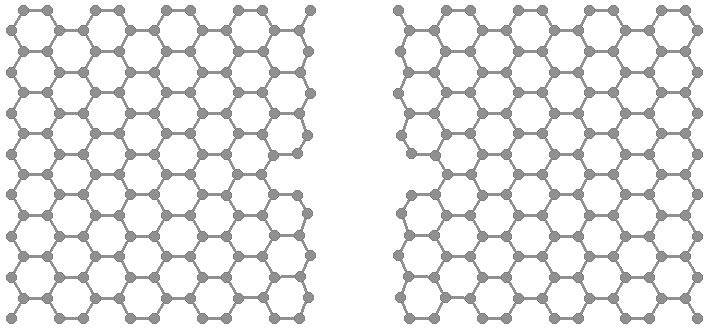
\includegraphics[width = .6\linewidth]{ADJUNTOS/roto_divacante.png}
%     \caption{Estructura final de la red de grafeno con dos vacantes. }
%     \label{fig:4.15}
% \end{figure}

% Como en casos anteriores con dopantes, la progresión de la energía es idéntica para la red de grafeno limpia como para las redes con defectos. La ruptura, sin embargo, se produce mucho antes en el caso de la red con defectos que en la red normal, alcanzándose en ambos casos a $3.0$ \AA \ de elongación con respecto a la longitud inicial. De hecho, esta ruptura se produce incluso antes que en el caso del boro ($4.2$ \AA) y del nitrógeno ($3.8$ \AA). Esto es debido a que, con dopantes, existen enlaces -- sin bien son débiles -- con el carbono que desaparecen al introducir una vacante (3 en el caso de la vacante, 6 con la divacante). Esto genera una gran inestabilidad estructural que favorece la ruptura de la red. Calculando el módulo de Young efectivo (en el caso de la divacante), obtenemos un valor de $Y = 0.892 \pm 0.016 $ TPa, ligeramente inferior al de la red ideal, que es una manifestación de esa inestabilidad estructural.    
